\documentclass[12pt, letter, oneside]{book}
\usepackage{fancyhdr, ifpdf}
\usepackage{float}
\usepackage{setspace}
\usepackage{color}
\usepackage{xcolor}
\usepackage{listings}
\usepackage{caption}
\usepackage[ampersand]{easylist}
\usepackage{amssymb}
\usepackage{pdflscape}
\usepackage{verbatim}
\usepackage{longtable}
\usepackage[margin=1cm]{caption}
\usepackage[top=1in, bottom=.75in, left=.7in, right=1in]{geometry}
\ListProperties(Hide=100, Hang=true, Progressive=3ex,Style*=$\bullet$ , Style2*=-- )

\definecolor{mygray}{rgb}{0.9,0.9,0.9}
\lstdefinestyle{customc}{
  backgroundcolor=\color{mygray},
  captionpos=b, 
  belowcaptionskip=1\baselineskip,
  breaklines=true,
  numbers=left,
  numberstyle=\footnotesize,
  %frame=L,
  xleftmargin=\parindent,
  language=C++,
  showstringspaces=false,
  basicstyle=\footnotesize\ttfamily,
  keywordstyle=\bfseries\color{green!40!black},
  commentstyle=\itshape\color{purple!40!black},
  identifierstyle=\color{black},
  stringstyle=\color{cyan}  
}

\lstset{escapechar=@,style=customc,tabsize=4}

%% some redefination of the headers and footers
\renewcommand{\chaptermark}[1]%
                 {\markboth{#1}{}}
\renewcommand{\sectionmark}[1]%
                 {\markright{\thesection\ #1}}
\lhead[\fancyplain{}{\thepage}]%
      {\fancyplain{}{\rightmark}}
\rhead[\fancyplain{}{\leftmark}]%
      {\fancyplain{}{\thepage}}
\cfoot{}
\sloppy

\ifpdf
   \usepackage[pdftex]{graphicx}
   \usepackage{rotating}
\else
   \usepackage{graphicx}
	\usepackage{rotating}   
\fi

\graphicspath{{./Figures/}}
\doublespacing

\begin{document}
\doublespace

\clearpage
\pagenumbering{arabic}

\setcounter{chapter}{0}


\newcommand{\pname}{Monte Carlo}

\chapter*{Parameter confidence estimation using the Monte Carlo bootstrap algorithm}
\setcounter{chapter}{1}
\emph{Get some confidence estimates}
\section{Introduction}
The Monte Carlo plugin is used to obtain estimates of the confidence limits for a model's parameters. This is in the context where experimental data exists and a parameter minimization method, such as Levenberg-Marquardt or Nelder-Mead has already been used in order to find a parameter minimum.

The Monte Carlo algorithm is used subsequently at this minimum and will give an estimate of parameter confidence limits corresponding to the variance in the original experimental data.

The plugin has properties such as the size of the Monte Carlo population, minimization algorithm to use (e.g. Nelder-Mead or Levenberg-Marquardt), and on output, confidence limits for each involved parameter.

Plugin properties are documented in more detail in the next section.

\begin{landscape}
\section{Plugin Properties}
Available properties in the \pname\ plugin are listed in the table below.

%\begin{table}[ht]
\centering % used for centering table
\begin{longtable}{p{4cm} l p{3cm}  p{10cm}} % centered columns

Property Name & Data Type & Default Value  & Description \\ [0.5ex] % inserts table
%heading
\hline % inserts single horizontal line
SBML                            &   string              & N/A    &   SBML document as a string. Model to be used by the \pname\ plugin. \\
ExperimentalData   				&	telluriumData 		& N/A    &   Input data.  \\
InputParameterList 				&	listOfProperties    & N/A    &   Parameters to estimate confidence limits for. \\
MonteCarloParameters 			&   listOfProperties 	& N/A    &   Parameters obtained from a Monte Carlo session. \\
ConfidenceLimits				&	listOfProperties	& N/A    &   Confidence limits for each fitted parameter. The confidence limits are calculated at a 95\% confidence level. \\
Experimental\-DataSelectionList & 	stringList			& N/A    &   Selection list for experimental data. \\
FittedDataSelectionList     	& 	stringList			& N/A    &   Selection list for model data. \\
NrOfMCRuns						&   int 				& N/A    &   Number of Monte Carlo data sets to generate and use.\\
MinimizerPlugin					&   string   			& N/A    &	 Minimizer used by the Monte Carlo Engine, e.g. "Levenberg\_Marquardt". \\

\hline %inserts single line
\caption{Plugin Properties}
\label{table:nmPluginProperties}
\end{longtable}
%\end{table}

\end{landscape}

\section{The \texttt{execute(bool inThread)} function}
The \verb|execute()| function will start the \pname\ algorithm. Depending on the problem at hand, the algorithm may run for a long time.

The \verb|execute(bool inThread)|, method supports a boolean argument indicating if the execution of the plugin work will be done in a thread, or not. Threading is fully implemented in the \pname\ plugin.

The inThread argument defaults to \textbf{false}.

Each generated Monte Carlo dataset is available in a file named, MCDataSets.dat (saved in current working directory).


\section{Plugin Events}
The \pname\ plugin uses all of the available plugin events, i.e. the \emph{PluginStarted}, \emph{PluginProgress} and the \emph{PluginFinished} events.

The available data variables for each event are internally treated as \emph{pass through} variables, so any data, for any of the events, assigned prior to
the plugins execute function (in the assignOn() family of functions), can be retrieved unmodified in the corresponding event function.

\begin{table}[ht]
\centering % used for centering table
\begin{tabular}{l l p{9cm}}

Event & Arguments & Purpose and argument types \\ [0.5ex] % inserts table
%heading
\hline % inserts single horizontal line
PluginStarted  	& 	void*, void*  & Signal to application that the plugin has started. Both parameters are \emph{pass through} parameters and are unused internally by the plugin.\\[0.5ex]
PluginProgress	& 	void*, void*  & Communicating progress of fitting. Both parameters are \emph{pass through} parameters and are unused internally by the plugin. \\[0.5ex]
PluginFinished	& 	void*, void*  & Signals to application that execution of the plugin has finished. Both parameters are \emph{pass through} parameters and are unused internally by the plugin.\\

\hline %inserts single line
\end{tabular}
\caption{Plugin Events}
\label{table:MCPluginEvents}
\end{table}

\section{Python example}
The following Python script illustrates how the plugin can be used.

\begin{singlespace}
\lstinputlisting[label=MonteCarloExample,caption={\pname\ plugin example.},language=Python]{Examples/telMonteCarlo.py}
\end{singlespace}

\begin{figure}[ht]
\centering
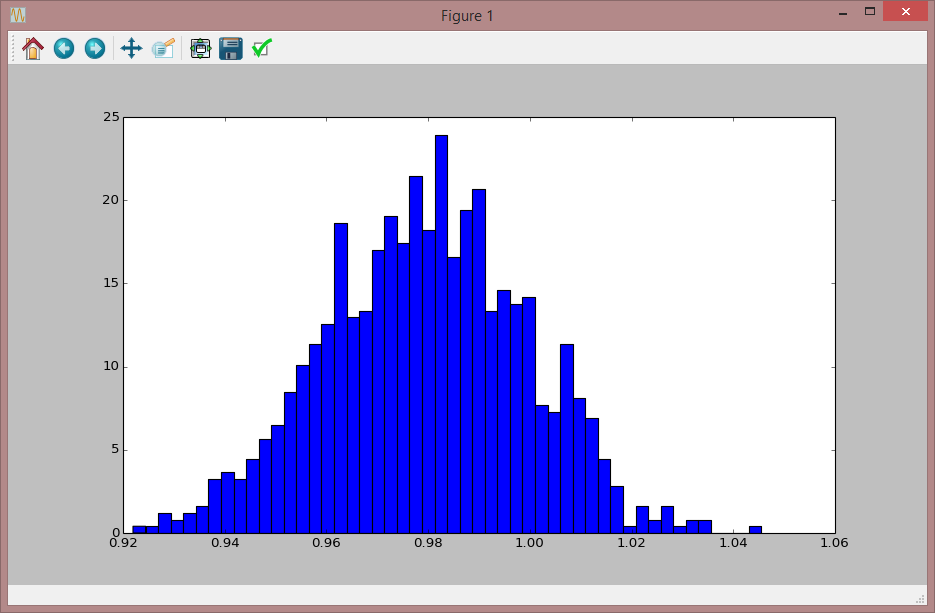
\includegraphics[width=\textwidth]{MonteCarloOutput.png}
\caption{Output for the example script above, using 1000 Monte Carlo runs. The histogram shows the distribution for the model parameter, 'k1'. The mean for the distribution was 0.980 and  obtained confidence limits were +/- 0.001.}
\label{fig:mcFig}
\end{figure}








\end{document}






